\documentclass[10pt]{beamer}

\usepackage{default}
\usepackage{minted}
\usepackage{graphicx}
\usepackage[utf8]{inputenc}
\usepackage[T1]{fontenc}
\usepackage{tikz}
\setminted{autogobble,tabsize=2,baselinestretch=1.0,escapeinside=&&}

\title{Elm}
\subtitle{Introdução e comparação com React/Redux}
\author{Rodrigo Stevaux @ Jaya Labs}

\begin{document}
	
\begin{frame}
\maketitle
\end{frame}


\begin{frame}[t]
	\frametitle{Elm: linguagem + arquitetura}
	\bigskip
	\hspace{-0.3cm}
\includegraphics[height=24pt]{logo.png}
	\begin{columns}[T]
		\begin{column}{0.5\textwidth}
			\begin{block}{Linguagem}
				\begin{itemize}
					\item Funcional pura
					\item Tipos estáticos c/ inferência
					\item Similar a F\#, Haskell e OCaml
					\item Especifica para SPA
				\end{itemize}
			\end{block}
		\end{column}
		\begin{column}{0.5\textwidth}
			\begin{block}{Arquitetura}
				\begin{itemize}
					\item Modelo: estado da aplicação
					\item Update: recebe comandos e atualiza modelo
					\item View: renderiza modelo em um DOM
					\item Equivalente a Redux + React + Thunk ou Saga
				\end{itemize}
			\end{block}
		\end{column}
	\end{columns}
	\bigskip
	Resultado: código fácil de manter e estender, clientes e devs mais felizes, menos bugs
\end{frame}

\begin{frame}
	\Huge{Arquitetura básica}
\end{frame}


\begin{frame}[fragile]
\frametitle{Modelos}
	O estado completo da aplicação é representado por um modelo, que geralmente é um record/struct com vários campos, e tudo é tipado:
	\bigskip
	\setminted{fontsize=\normalsize}
    \begin{minted}{elm}
type alias Model = {
	running : Bool,
	elapsed : Float,
	pastLaps : List Float 
}
    \end{minted}
    \bigskip
    Em um cronômetro, o estado é se o relógio está parado ou correndo, qual o tempo acumulado na volta atual, e quais os tempos das voltas passadas.
\end{frame}

\begin{frame}[fragile]
	\frametitle{Mensagens}

	Mensagens carregam comandos para o aplicativo fazer qualquer coisa útil: alterar alguma variável do estado, fazer algum request para falar com alguma API, aumentar um counter, etc.
	
	\bigskip
	\setminted{fontsize=\normalsize}
	\begin{minted}{elm}
		type Msg = 
			  Start 
			| Stop
			| Reset
			| Lap
			| Tick Time
	\end{minted}

\end{frame}


\begin{frame}[t, fragile]
	\frametitle{Update}
	Atualizamos o estado da aplicação enviando \mintinline{elm}{Msg} para o \mintinline{elm}{update}, que transforma o \mintinline{elm}{model} anterior e retorna um novo:
	\setminted{fontsize=\normalsize}
	\begin{minted}{elm}
	update : Msg -> Model -> Model
	update msg model =
		case msg of
			Start -> { model | running = True }
			Stop  -> { model | running = False }
			Reset -> { model | elapsed = 0 }
		  -- h :: t coloca o elemento h na frente da lista t				
			Lap   -> { model | laps = model.elapsed :: model.laps, 
			                   elapsed = 0 }
			Tick time -> { model | elapsed = Time }
	\end{minted}
	\bigskip
	Isso é bom, pois em um lugar só podemos ver tudo que pode acontecer com o modelo, e, com os tipos, o Elm só compila a aplicação se todas as mensagens forem tratadas!
\end{frame}


\begin{frame}[t, fragile]
	\frametitle{Views}
	\bigskip
	As views no Elm são apenas funções que geram HTML a partir do modelo (Os equivalentes no React seriam componentes puros.)
	\bigskip
	\begin{minted}{elm}
	view model = div [] [
		div [] [h1 [] [text <| format "%M:%H:%S" model.elapsed]],
		, div [] [b [] [text "Laps:"]]
		, div [] (List.map viewLap model.laps)
		, div [] [button [onClick Start] [text "Start"]]
		, div [] [button [onClick Stop] [text "Stop"]]
	]
	viewLap lap = div [] [text <| format "%M:%H:%S" model.elapsed]
	\end{minted}
	\bigskip
	Esse \mintinline{elm}{onClick Start} faz uma mensagem \mintinline{elm}{Start} chegar ao \mintinline{elm}{update}.
\end{frame}

\begin{frame}[t, fragile]
	\frametitle{Subscriptions}
	\bigskip
	O Elm tem um conceito de "subscriptions" para ouvir eventos do browser como timers, mouse e keyboard, por exemplo. Conforme o modelo mudar, as subsriptions tambem podem mudar, como ilustrado na função seguinte:
	\bigskip
	\begin{minted}{elm}
	subscriptions : Model -> Sub Msg
	subscriptions model =
		if model.running then
			Time.every (20 * millisecond) Tick
		else
			Sub.none
	\end{minted}
	\bigskip
	Cada subscription envia uma \mintinline{elm}{Msg} para o \mintinline{elm}{update}. Se o cronometro está ligado, queremos ser avisados com a mensagem \mintinline{elm}{Tick} no \mintinline{elm}{update} a cada 20 ms
\end{frame}

\begin{frame}[t, fragile]
	\frametitle{E como juntar as partes?}
	\medskip
	A aplicação tem uma função main, que usa a função program, para juntar as partes da arquitetura:
	\begin{minted}{elm}
		main = 
			program init view update subscriptions
			
		init = ..., view = ...
		update = ..., subscriptions = ...
	\end{minted}
	\medskip
	Isto tudo é compilado para um único .JS para incluirmos em um HTML. Elm não precisa ser usado na página toda.
	\medskip
	\begin{minted}{html}
	<script src="app.js"/>
	<div id="root"></div>
	<script>
		var root = document.getElementById("root");
		var app = Elm.Main.embed(root);
	</script>
	\end{minted}
\end{frame}

\begin{frame}
	\Huge{APIs: usando HTTP e JSON}
\end{frame}

\begin{frame}[fragile]
\frametitle{JSON: transformando em valores do Elm}
Decode de JSON é representado de forma type-safe:
\\
\begin{minted}{elm}
    type Decoder a = Json.Value -> a

    decodeValue : Decoder a -> Value -> Result String a
\end{minted}
\
\\
Ou seja: para decodificar um valor JSON para um valor Elm nós aplicamos um Decoder a uma String, e temos como resultado ou uma mensagem de erro ou um valor do tipo \verb|a|
\end{frame}

\begin{frame}[fragile]
    \frametitle{Exemplo}
    Tem muita coisa funcional acontecendo atrás disso, mas para os usuários basta usar como uma DSL:
    \begin{minted}{elm}
    import Decode as D

    type alias Model = { elapsed, running, laps }
    
    decodeModel : D.Decoder Model
    decodeModel =
        D.map2 Todo
            (D.field "elapsed" D.float)
            (D.field "running" D.bool)
            (D.field "laps" (D.list D.string))
    \end{minted}
\end{frame}

\begin{frame}[t]
	\frametitle{HTTP}
	\bigskip
	As chamadas HTTP no Elm são assíncronas e se encaixam na arquitetura através do \mintinline{elm}{update}:
	\bigskip
	\begin{itemize}
		\item Uma chamada HTTP é um \mintinline{elm}{Cmd Msg}, que é executado pelo run-time do Elm
 		\item Quando chegar a resposta, o run-time envia uma \mintinline{elm}{Msg} para \mintinline{elm}{update}
	\end{itemize}
	\bigskip
	A chamada é organizada em 3 partes:
	\bigskip
	\begin{enumerate}
		\item A url e o verbo HTTP
		\item Um decoder para a resposta com tipo \mintinline{elm}{Decoder a}
		\item Um caso de \mintinline{elm}{Msg} com um campo \mintinline{elm}{Result Http.Error a}
	\end{enumerate}
\end{frame}

\begin{frame}[fragile]
	\frametitle{Exemplo}
	\begin{minted}{elm}
	
		getAppState : Cmd Msg
		getAppState =
			let req = Http.get "api.webpage.com/states/" decodeModel
			in Http.send req ModelFromServer
	
		type Msg = 
			...
			| ModelFromServer (Result Http.Error Model)
				
		update msg model =
			case msg of
				...
				ClickRestore -> (model, getAppState)
				ModelFromServer (Ok mod) -> (mod, Cmd.none)
				ModelFromServer (Err err) -> ...
		
	\end{minted}
\end{frame}

\begin{frame}
	\Huge{Demo}
\end{frame}

\begin{frame}
	\frametitle{Por quê usar Elm se parece tanto com React?}
	Elm gera software mais correto, robusto e gera menos stress para desenvolvedores e clientes.
	\medskip
	\begin{itemize}
		\item Os tipos deixam tudo mais seguro, checado pelo compilador
		\item O compilador é um guia para o processo de desenvolvimento
		\item Refatorar é muito mais fácil com tantos checks no compilador
		\item Async done right
		\item Build system super simples - um só comando
	\end{itemize}
	\medskip
	O jeito mais fácil é demonstrar isso em uma sessão de live coding
\end{frame}

\begin{frame}
	\huge Backup
\end{frame}

\begin{frame}
	\frametitle{Tradicional}
	\begin{center}
		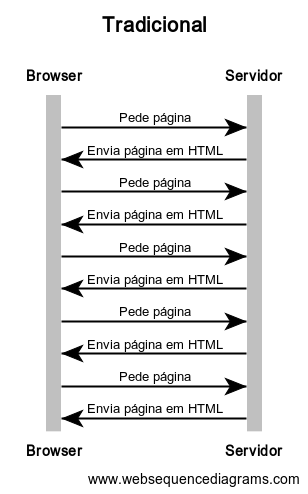
\includegraphics[height=70mm]{tradicional.png}
	\end{center}
\end{frame}

\begin{frame}
	\frametitle{Single-page applications}
	\begin{center}
		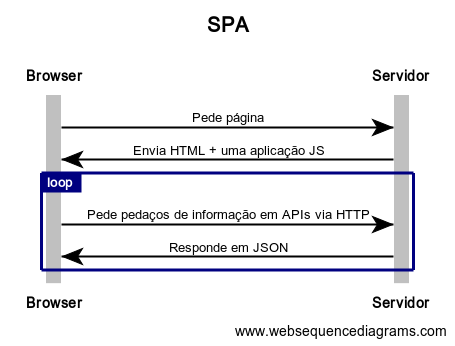
\includegraphics[width=80mm]{spa.png}
	\end{center}
\end{frame}

\end{document}
